\documentclass[12pt, oneside]{article}
\usepackage[letterpaper, margin=1in, headsep=0.5in]{geometry}
\usepackage[english]{babel}
\usepackage[utf8]{inputenc}
\usepackage{amsmath}
\usepackage{amsfonts}
\usepackage{amssymb}
\usepackage{tikz}
\usetikzlibrary{quotes, angles}
\usepackage{graphicx}
%\usepackage{pgfplots}
%\pgfplotsset{width=10cm,compat=1.9}
%\usepgfplotslibrary{statistics}
%\usepackage{pgfplotstable}
%\usepackage{tkz-fct}
%\usepackage{venndiagram}

\usepackage{fancyhdr}
\pagestyle{fancy}
\fancyhf{}
\rhead{\thepage \\Name: \hspace{1.5in}.\\}
\lhead{BECA / Huson / 11.1 IB Math SL\\4 October 2018}

\renewcommand{\headrulewidth}{0pt}

\begin{document}
\subsubsection*{Unit 1 Test: Function Operations}
Answer on loose leaf paper in pen, or, for the graphs, on graph paper in pencil. Show working for all problems. %State answers exactly or to three significant figures.
  \vspace{0.5cm}
  \begin{enumerate}

    \item For the function $f(x) = 2x+3$
    \begin{itemize}
        \item[(a)] What is the value of $f(-1)$?
    	\item[(b)] Solve for $x$ if $f(x)=0$.
    	\item[(c)] Find  $f(3-2x)$.
    	\item[(d)] Find the inverse of $f(x)$,  $f^{-1}(x)$.
    \end{itemize}

    \item For the functions $f(x) = 1-x^2$ and $g(x) = x-4$
    \begin{itemize}
        \item[(a)] What is the value of $g(5)$?
    	\item[(b)] Find $(f\circ g)(5)$.
    	\item[(c)] Find $(f\circ g)(x)$.
    \end{itemize}

    \item Find the inverse of $\displaystyle f(x)= \frac {2x-2}{3}$

    \item For the functions defined by $f(x) = 2x$ and $g(x) = x+4$
    \begin{itemize}
        \item[(a)] Find an expression for $(f\circ g)(x)$.
    	\item[(b)] Find an expression for $(g\circ f)(x)$.
    	\item[(c)] Solve $(f\circ g)(x)=(g\circ f)(x)$.
    \end{itemize}

    \item Write down the domain and range of $f(x)= x^2-6$

    \item For the function shown in the graph below,
    \begin{itemize}
      \item[(a)] Write down the equations for the asymptotes.
    	\item[(b)] Write down the domain and range of the function.
    \end{itemize}


    \item Using a GDC to analyze the function $\displaystyle f(x)= \frac {2x+1}{x+3}$
    \begin{itemize}
        \item[(a)] Write down the equations for the asymptotes.
    	\item[(b)] Write down the domain and range of $f(x)$.
    \end{itemize}

\newpage
    \item Graph the function $f(x)=x^2+2x+2$ over the domain $-1 \leq x\leq 1$.
    \begin{itemize}
        \item[(a)] Mark points on the function representing $f(-1)=1$ and $f(1)=5$. Label them as coordinate pairs.
    	\item[(b)] Graph and label the inverse of $f$, $f^{-1}(x)$, on the same axes over the domain corresponding to the range of $f$ graphed. Mark the inverses of the points named in part (a), labeling them as coordinate pairs.
    	\item[(c)] Write down the domain and range of $f^{-1}(x)$ in the space below. \vspace{2cm}
    \end{itemize}
    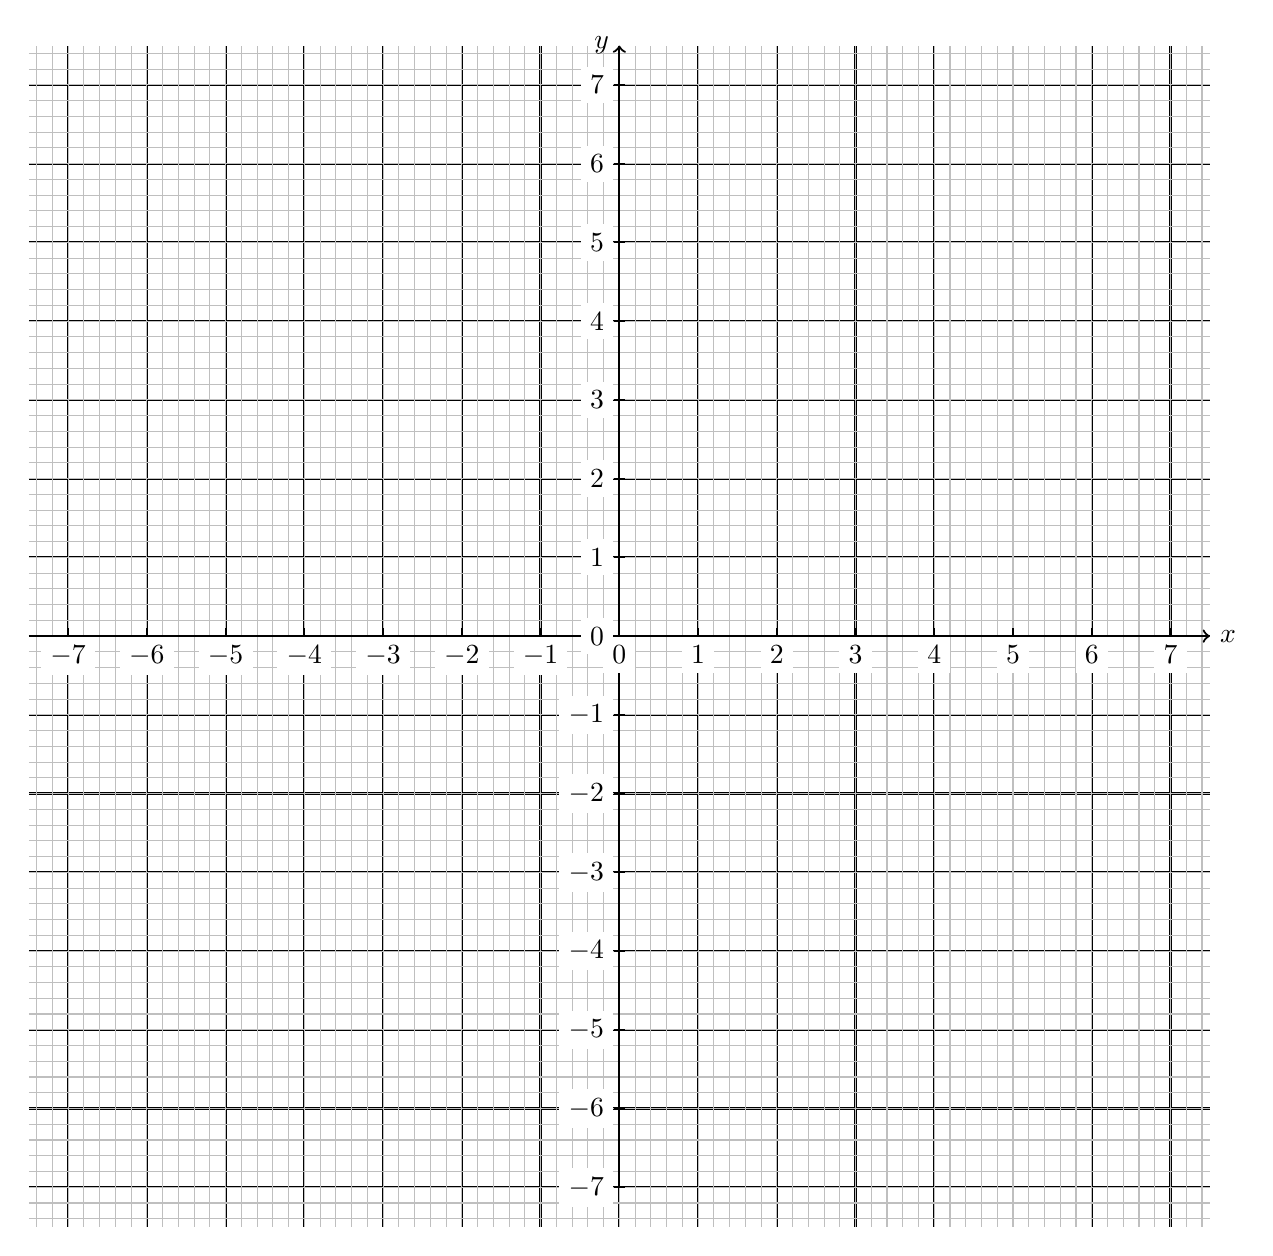
\begin{tikzpicture}[scale=1] %grid with numbered axes, IB cm paper.
      %\clip (-5.5, -1.5) rectangle (5.5, 7.5);
      \draw [thick, color=black,, xstep=1.0cm,ystep=1.0cm] (-7.5,-7.5) grid (7.5,7.5);
      \draw [thin, color=lightgray,, xstep=0.2cm,ystep=0.2cm] (-7.5,-7.5) grid (7.5,7.5);
      \draw [thick, ->] (-7.5,0) -- (+7.5,0) node [right] {$x$};
      \draw [thick, ->] (0,-7.0) -- (0,7.5) node [left] {$y$};
      \foreach \x in {-7,...,7}
        \draw[shift={(\x,0)},color=black] (0pt,-3pt) -- (0pt,3pt) node[below=3pt, fill=white]  {$\x$};
      \foreach \y in {-7,..., 7}
        \draw[shift={(0,\y)},color=black] (2pt,0pt) -- (-2pt,0pt) node[left, fill=white]  {$\y$};

      %\draw [<->, thick] plot[domain= -5:5] (\x, {(3*\x+1)/(\x-2)});
    \end{tikzpicture}

    %missing: identifying a function vs relation,

  \end{enumerate}
\end{document}

\newpage


\begin{tikzpicture}[scale=1] %grid full page without axes, IB cm paper.
  \draw [thick, color=black,, xstep=1.0cm,ystep=1.0cm] (0,0) grid (15,20);
  \draw [thin, color=lightgray,, xstep=0.2cm,ystep=0.2cm] (0,0) grid (15,20);
\end{tikzpicture}
